\documentclass[letterpaper]{article}
\usepackage{natbib,alifeconf}
%\usepackage{hyperref}
\usepackage{todonotes}
\usepackage{epstopdf}
\usepackage{soul}

\usepackage[flushleft]{threeparttable}
\usepackage{subcaption}
\usepackage{booktabs}
\setcounter{tocdepth}{3}
\usepackage{array}
\usepackage{float}
\usepackage{dirtytalk}
  \usepackage[font=small]{caption}

\delimitershortfall-1sp
\newcommand\abs[1]{\left|#1\right|}

\title{Evolution of Heterogeneous Cellular Automata in Fluctuating Environments}
\author{David Medernach$^{1}$, Simon Carrignon$^{2,3}$, Ren\'{e} Doursat$^{4}$, Taras Kowali, Jeannie Fitzgerald$^1$ \and Conor Ryan$^1$ \\
\mbox{}\\
$^1$BDS Group - University of Limerick  \\
$^2$Barcelona Supercomputing Center \\
$^3$Complex System Lab Universitat Pompeu Fabra \\
$^4$Manchester Metropolitan University \\
david.medernach@ul.ie}

\begin{document}
\maketitle

\begin{abstract}
The importance of environmental fluctuations in the evolution by natural selection of living organisms has been widely noted by biologists and linked to many important characteristics of life such as: modularity, plasticity, genotype size, mutation rate, learning or epigenetic adaptations. In artificial life simulations, however, environmental fluctuations are usually seen as a nuisance rather than an essential characteristic of evolution. HetCA is a heterogeneous cellular automata characterized by its ability to generate open-ended long-term evolution and ``evolutionary progress''. In this paper, we propose to measure the impact of different types of environmental fluctuations in HetCA. Our results indicate that environmental changes induce mechanisms analogous to epigenetic adaptation or multilevel selection. This is particularly prevalent in two of the tested fluctuation schemes, which involve a round-robin inhibition of certain cell types, where a phenotypic selection seems to occur.
\end{abstract}

\section{Introduction}\label{sec:intro}

Environmental changes may include cyclic events such as seasonal changes or a daily cycle of light and darkness, occasional changes such as the introduction of new predator or the potential for a new source of food, or much more radical modifications such as environmental stresses induced by climate change.

Since works such as~\citep{levins1968evolution} or more recently~\citep{jablonka2014evolution}, as well as with the attempt made to integrate the epigenetic (EIS), developmental ("Evo-Devo"~\citep{muller2007evodevoextendingtheevolutionarysynthesis}) and environmental ("Niche Construction"~\citep{laland2016anintroductiontonicheconstructiontheory} dimensions to evolutionary biology, the emphasis has been put on the importance of such change on the course of the evolution by natural selection of living beings. Through these and other works, they have been linked to many central mechanisms of evolution. Modularity, plasticity~\citep{west2005developmental}, size of the genotype, mutation rate and evolvability are some of the most discussed example. 

For \cite{jablonka2014evolution}, changeable environments will unmask variations in the capacity of individuals to make adjustments to changed conditions and therefore promote plasticity. They advance that \say{For a lineage in a constantly changing environment, switching among several alternative heritable states was probably an advantage. While cells in one state survived in one set of conditions, those in other states did better in different circumstances.}\emph{(ibid. p. 318)}. Following that line of thought, constantly changing environment or cycling variations might explain the origin of the Epigenetic Inheritance Systems~\citep{heard2014transgenerationalepigeneticinheritancemythsandmechanisms}, as epigenetic mutations are more reversibles and occur more frequently than genetic mutations. 

To illustrate that, \cite{lachmann1996inheritance} have modelled the effects of cycling variations, such as seasonal or daily cycles, on phenotypical inheritances. Their model predicted that indeed when the investigated cycles are longer than the reproductive cycle but relatively short otherwise, heritable variations produced by non-DNA inheritance systems are likely to be observed. 

In parallel to such studies, a proportion of existing works in artificial life, especially in evolutionary robotics~\citep{floreano2000evolutionary}, considers the issue of environmental variations. Some work in this literature have explicitly define the environment as a driving evolutionary force~\citep{bredeche2012environmentdrivenopenende}. %However and as far as we know, a significant majority of the works in that field still consider environmental changes only as a problem to be solved and nobody has systematically studied the general properties induced by environmental fluctuations over evolutionary dynamics.  %However, it is probably fair to say that, a significant majority of these previous work has either focused on aspects such as normal spatial variation, or has viewed environmental change as a problem to be solved.

Other, such as~\cite{lipson2002origin}, demonstrated a correlation between the modularity and the rate of change of the environment resources, while \cite{yu2007program} observed that populations exploit neutrality to cope with environmental fluctuations and therefore evolve some sort of evolvability under two alternating objective functions. Both of these two last simulations used Genetic Programming~(GP) and employed explicit fitness functions.

We wish to study effects of such fluctuations in a model closer to the living world without using any explicit fitness function. We then propose an open ended experimental setup that allows to systematically and quantitatively measure the influence of cyclic environmental fluctuations on the course of the evolution of a Cellular Automata (CA). We show that such fluctuations lead to the emergence of processes similar to those exhibited by epigenetic inheritance systems.

The paper is organized as follow. First the general mechanisms of HetCA model are described. Then implementation of environmental fluctuations in HetCA is detailed. Afterward we specify the computer experimental setup used to study environmental fluctuations. Later we report experimental results and discuss the implications of these results. Finally we propose a qualitative analysis and conclude.



%\section{Background}\label{sec:bground}
%
%In~\citep{lipson2002origin} Lipson demonstrated a correlation between the modularity and the rate of change of the environment resources. While in \citep{yu2007program} Yu used observed that populations exploit neutrality to cope with environmental fluctuations and therefore evolve some sort of evolvability under two alternating objective functions. Both of these simulations used Genetic Programming~(GP) and employed explicit fitness functions.



\section{HetCA}\label{sec:hetca)}
HetCA is based on classical two-dimensional cellular automata~(CA), but has several added features: cells have \emph{age}, \emph{decay} and \emph{quiescence} properties; cells utilize a heterogeneous transition function inspired by linear genetic programming~(LGP); and there exists a notion of genetic transfer of transition functions between adjacent cells.

HetCA exhibits long term phenotypic dynamics, sustains a high level of variance over very long runs and displays greater behavioural diversity than classical cellular automata\citep{medernach2013long}. HetCA also exhibits Evolutionary Progress (EP) according to the three criteria : robustness, size and density of generated genotypes\citep{medernach2015evolutionary}, using Shanahan's definition of EP \citep{shanahan2012evolutionary}.

Moreover, some emergent properties of HECA are similar to two of the five major eukaryotic innovations which do not appear to have direct prokaryotic predecessors defined in~\citep{smith1997major} as : the eukaryotic chromatin remodelling machinery; the cell cycle regulation systems; the nuclear envelope, the cytoskeleton; and the apoptosis apparatus\citep{koonin2002origin}. Indeed, in HetCA, the loss of the genotype of the cell as it turns to the quiescent state may seem similar to apoptosis while survival strategies such as the ones depicted in Figure~\ref{foursteps} might akin cell cycle regulation systems.
Finally, controversy over the units of selection\footnote{Genotype selection, Phenotype selection, epigenetic selection, comportemental selection, multilevel selection...} in evolutionary biology~\citep{okasha2006evolution} are numerous and date back to the origins of this field of research and there is potentially several units of selection in HetCA: genotypic selection of the transition rules but also phenotypic selection of cell group replicating patterns that one can also find in cellular automata such as game of life.  This issue is important when one is interested in environmental fluctuations because, as mentioned in introduction, it is anticipated that the existence of frequent environmental fluctuation could promote phenotypic selection compared to genotypic selection.




\section{Experimental Setup}\label{sec:exsetup}
As in the previous version of HetCA \citep{medernach2013long}, the genotype of an individual consists of its transition rules encoded in a custom CA-LGP program using the function set listed in Table~\ref{funcSet}. Such a program maps the space of neighborhood states to a new cell state, while providing an evolvable representation framework based on an alphabet of elementary functions. Individual genotypes are modified by micro-mutations (change in one component of a statement) and macro-mutations (addition or removal of an entire statement) of the corresponding CA-LGP programs.
 
\begin{table}
\scriptsize
\centering
  \begin{tabular}{l>{\centering}p{0.6\columnwidth}}
  \toprule%
    \textbf{op. name}	& \textbf{action} on inputs $(x,y)$\tabularnewline
 \toprule%   
    abs			& $|x|$ \tabularnewline
    plus		& $x+y$ \tabularnewline
    delta		& 1, if $|x-y| < 1/10,000$; 0 o.w. \tabularnewline
    dist		& $|x-y|$ \tabularnewline
    inv			& $1-x$ \tabularnewline
    inv2		& safeDiv($1, x$) \tabularnewline
    magPlus		& $|x+y|$ \tabularnewline
    max			& $\max \{x,y\}$ \tabularnewline
    min			& $\min \{x,y\}$ \tabularnewline
    safeDiv		& $x/y$ if $|y| >  1/10,000$; 1 o.w. \tabularnewline
    safePow		& $x^y$, if defined; 1 o.w. \tabularnewline
    thresh		& 1, if $x > y$; 0 o.w.\tabularnewline
    times		& $xy$ \tabularnewline
    zero		& 1, if $|x| < 1/10,000$; 0 o.w. \tabularnewline
\bottomrule%
  \end{tabular}
    \caption{\textbf{Function set}. \label{funcSet}}
\end{table}

Previously, the new genotype of a living cell $c$ during genetic transfer was chosen randomly among candidate neighboring genotypes according to a uniform distribution. In the present study, to introduce environmental variations we vary the likelihood of propagation of a genotype according to its cell state $S_c$. In this new setup, the probability $P(c)$ of a candidate genotype to be selected becomes $P(c)=K(S_c)/\sum_{i=1}^{n} K(S_{c_i})$, where $K(S)$ the state distribution and $n$ the number of candidate genotypes. Therefore an environment $E$ is characterized by the propagation probabilities of the 5 living states: $E=\{K(S_1),...,K(S_5)\}$. To mimic environmental fluctuations we initialize the simulation with $K(S_i)=1$ everywhere, then regularly modify those values every $f$ iterations starting from iteration 3,000 of the CA. We introduce three types of environmental fluctuations (Table~\ref{tab:environments}):

\newcommand*{\TitleParbox}[1]{\parbox[l]{10cm}{\raggedright #1}}%
\begin{table*}
\caption{Stable and fluctuating environments.\label{tab:environments}}
\scriptsize

\begin{tabular}{lccccl}
\toprule%
{\textbf{Name}} & {\textbf{Short Name}} & \textbf{Cycles}\tnote{a} & \textbf{Transitions}\tnote{b} &\textbf{Environment list: propagation probabilities $E = \{K(S_1),...,K(S_5)\}$ of the living types} \tabularnewline
\toprule%
\textbf{Stable Environment} & (SE) & NA & NA & \TitleParbox{$\{1,1,1,1,1\}$} \tabularnewline

\textbf{Short-cycle Fluctuations} & (ScF) & 100 & 1 & \TitleParbox{$\{0,0,1,1,1\}$, $\{1,1,1,0,0\}$} \tabularnewline

\textbf{Light Fluctuations} & (LF) & 5,000 &  1 & \TitleParbox{$\{1,1,1,1,0\}$, $\{1,1,1,0,1\}$, $\{1,1,0,1,1\}$, $\{1,0,1,1,1\}$, $\{0,1,1,1,1\}$, $\{1,1,1,1,1\}$}\tabularnewline
    
\textbf{Strong Fluctuations} & (SF) & 5,000 & 1 & \TitleParbox{$\{0,0,1,1,1\}$, $\{1,1,1,0,0\}$, $\{0,1,0,1,1\}$, $\{1,0,1,1,0\}$, $\{0,1,1,0,1\}$, $\{1,1,0,1,0\}$, $\{1,0,1,0,1\}$, $\{0,1,1,1,0\}$, $\{1,0,0,1,1\}$, $\{1,1,0,0,1\}$, $\{1,1,1,1,1\}$} \tabularnewline

%\textbf{Gradual Fluctuations} & (GF) & 5,000  & 60 & \TitleParbox{$\{0,0,1,1,1\}$, $\{1,1,1,0,0\}$, $\{0,1,0,1,1\}$, $\{1,0,1,1,0\}$, $\{0,1,1,0,1\}$, $\{1,1,0,1,0\}$, $\{1,0,1,0,1\}$, $\{0,1,1,1,0\}$, $\{1,0,0,1,1\}$, $\{1,1,0,0,1\}$, $\{1,1,1,1,1\}$} \tabularnewline

\bottomrule%
\end{tabular}%
\end{table*} 

\emph{Short-cycle fluctuations (ScF)} consist of alternating between two environments every $f$ iterations of the CA. We choose $f=100$ to remain within the range of frequency described by \citet{lipson2002origin} and \citet{yu2007program}. Here we consider that a successful reproductive cycle for a cell involves passing through the quiescent state. This should take between 2 iterations (alternating between quiescent and living) and 7 iterations (after which a living cell decays and can no longer receive a genotype for a long period of time).

\emph{Light fluctuations (LF)} consist of alternating between 6 environments every $f=5,000$ iterations. The first 5 environments each prohibit a different living state (out 5 possible ones) from spreading its genotype; the last one gives an equal chance to all living states.

\emph{Strong fluctuations (SF)} consist of alternating between 11 environments every $f=5,000$ iterations. The first 10 environments each prohibit a different pair of living states (out 10 possible ones) from spreading their genotypes; the last one gives an equal chance to all pairs.

%\noindent \emph{Gradual Fluctuation}: is similar to strong fluctuations except that it includes a transition phase of $T=60$ iterations in between two environments where likelihood of spread of state values progressively switch from the value a previous environment to the ones of the new environment. Over this phase the state spreading is defined by the following formula : $K(S,t)=K_p(S) \times (T-t) + K_{p+1}(S) \times t$ where $t$ is the number of iterations completed since the beginning of the transition phase; $K_p(S)$ and $K_{p+1}(S)$ are likelihood of state spread $S$ for the current environment and the next environment respectively.

The rationale behind ScF is their analogy with circadian rhythms in certain bacteria. The intention is to mimic the highly regular cycles during which these organisms have enough time to reproduce repeatedly. LF, by contrast, are more similar to seasonal fluctuations, while SF resemble ecological crises. However, owing to the variety of both biological temporal rhythms and reproductive cycles, the relevance of these analogies remains rather limited.

%\subsection{Common Settings}\label{sec:commonset}


\section{Simulations}\label{sec:method}

For each form of environmental fluctuation and the stable non fluctuating environment we performed 50 simulations which make a total of $4\times50=200$ runs. Each run last 500000 iterations with the parameters listed in Table~\ref{settings}. In following section we report average value with standard deviations.

\begin{table}
\scriptsize
\centering
\begin{tabular}{l>{\centering}p{0.2\columnwidth}}\toprule%
Parameter & Value \tabularnewline
\toprule%
Number of living states & 5\tabularnewline
Successive living iterations before decay & 7\tabularnewline
Number of iterations for decay & 375-1875\tabularnewline
Direct transition to decay & enabled\tabularnewline
Size of the grid & 500x500\tabularnewline
Grid boundaries & toric grid\tabularnewline
Transition Rule~(TR) & CA-LGP\tabularnewline
Maximum (TR) size & 50 program statements\tabularnewline
Genotype copy neighbouring  & Von Neumann \tabularnewline
Transition rule neighbouring & Moore\tabularnewline
\bottomrule%
\end{tabular}
\caption{ \textbf{HetCA parameters}.}
  \label{settings}
\end{table}

\subsection{Genotype Size}
We use the number of program statements ($n_{prog}$) as a measure of the genotype size and compute the average size of all the current genotypes of a run every 2500 iterations. We then report the average and standard error among all the fifty runs sharing the same settings.

\subsection{Changes induced by environmental fluctuation}
If, as postulated in \citep{jablonka2014evolution}, the introduction of environmental changes leads to the selection of plasticity or to the emergence of phenotypic selections\footnote{Similar to the epigenetic inheritance system} using easily reversible phenotypic mutations, then phenotypes from different individuals of the same lineage observed while environmental conditions are similar should be relatively close even though individuals from their lineage evolved in other environmental conditions between these measures. While, if the adaptation to each environmental change is done exclusively through the selection of classical irreversible genotypic mutations, these phenotypes shall be quite different, despite the potential evolutionary convergence. That is why we want to develop a metric to measure phenotypic proximity between two iterations of the CA. To do this we simply compare the proportions of living cells in different states among the possible states. The phenotypic difference $\sigma(t_1,t_2)$ between two iterations $t_1$ and $t_2$ is then calculated as:
$$\sigma(t_1,t_2) = \sum_{s=1}^5 \abs{ \frac{N(s,t_1)}{N(t_1)}-\frac{N(s,t_2)}{N(t_2)}}$$ where $N(s,t)$ is the number of cells at the state $s$ for iteration $t$ and $N(t)=\sum_{s=1}^5 N(s,t)$ is the total number of living cells.

Every 5000 iterations $t$ of the CA we perform two phenotypic comparison with an iteration $t'$ such as $t'\in[t-55000;t-60000]$. The first phenotypic comparison aims to compare two similar environment and therefore we choose $t'$ such as $E(t')=E(t)$. The second phenotypic comparison aims to compare two disimilar environment and therefore we choose $t'$ such as $E(t')=E(t+f)$.  

\subsection{Diversity}
We use the true diversity index of order two to measure phenotypic and genotypic diversity at every iteration $t$ of the CA. Phenotypic diversity is therefore: $$^2D_p(t)=\left(\sum_{s=1}^5 \left(\frac{N(s,t)}{N(t)}\right)^2\right)^{-1}$$ while genotypic diversity is: $$^2D_g(t)=\left(\sum_{g=1}^{K(t)} \left(\frac{N(g,t)}{N(t)}\right)^2\right)^{-1}$$ with $K(t)$ number of distinct genotypes for iteration $t$ and $N(g,t)$ number of cells sharing the genotype $g$ at iteration $t$, note that $N(t)=\sum_{s=1}^5 N(s,t)=\sum_{g=1}^{K(t)} N(g,t)$.

\subsection{Homogenous Test}
We also collect the \emph{most common genotype}~(most frequently occurring) in iterations 2500\footnote{\citep{medernach2015evolutionary}  has shown that the most common genotypes during the first iterations of HetCA were unlikely to have a viable survival strategy, therefore we chose to collect genotypes from iteration 2500}, 102500, 202500, 302500, 402500 and 500000. We tested all genotypes collected in homogeneous simulations, i.e. without mutation and where all cells are initialized with the tested genotype. We then tested each collected genotype in every four environment used, thus performing $4\times50\times6\times4=4800$ runs. We set the maximum duration of these runs to 60000 iterations so that runs performed with \emph{Strong Fluctuations} last long enough to go through all environments. Sometimes the genotype is not adapted to the environment and living cells extinct\footnote{By all turning to decay or quiescent state.} before the end of the 60000 iterations. We consider an Homogenous test to be successful if living cells doesn't extinct before 60000 iterations. We report the success rate of those simulations and the ending iterations of the runs that fail o reach iteration 60000. 

\subsection{Regular phenotype characterization and Phenotype disturbance} 
In HetCA, to survive in the long term the genotypes must regularly release cells by transforming them into quiescent cells without genotypes. This generates patterns and cycles which are quite easy to observe in homogeneous simulations where a single genotype is tested as shown in Figure~\ref{foursteps}~(a), but also observable, although with more difficulty, in normal, heterogeneous, HetCA simulations as seen in Figure~\ref{foursteps}~(b).That is why, to characterize phenotypes, we found it useful to measure these cycles as well as out-of regularities. At every iteration $t>8$ of the homogenous genotype test, we compare the states $S_t$ and $S_{t-1}$ of each cell to their anterior state during the eight previous iterations of the CA. We then measure whether this sequence of two states is repeated during these eight previous iterations, and if so what is its periodicity $p$ such as $p=\min p \in [2;7], S_t=S_{t-p} \wedge S_{t-1}=S_{t-1-p}$. We use here a sequence of two states because, if the genotype of a cell adopts a stable strategy, i.e. repeats a sequence of states, this sequence must contain a minimum of two states in order to ensure the survival of the genotype -- the quiescent state and one of the living states. We have chosen to limit ourselves to a comparison of the eight previous iterations to reduce the computational cost and because the limit of the seven consecutive live iterations before decay involves, for a successful regular phenotype, a maximum periodicity of seven iterations for the quiescent state. We perform this measure only if there is at least a living state among the last two states and no state decay. We then report, for each iteration $t$ of the CA, the phenotype disturbance $$P(t) = \sum_{p=1}^7 \abs{ \frac{N(p,t)}{N(t)}-\frac{N(p,t-1)}{N(t-1)}}$$ with $N(p,t)$ total number of cell with $p$ periodicity for iteration $t$. This measure is quite rough but it is interesting because here, unlike phenotypic difference, it is not directly based on the states of the cells and therefore seems less available able to be directly correlated to state's likelihood of spread.
 
\begin{figure}[h]
\centering
\begin{tabular}{cc}
    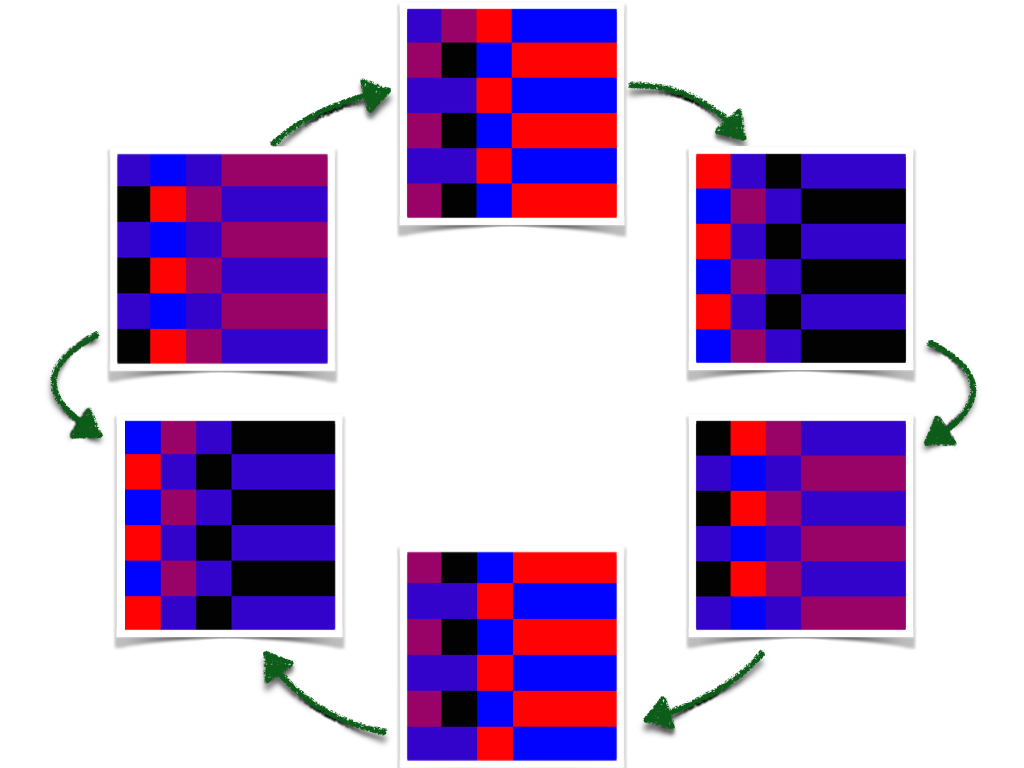
\includegraphics[width=0.45\columnwidth]{img/4steptransition}& 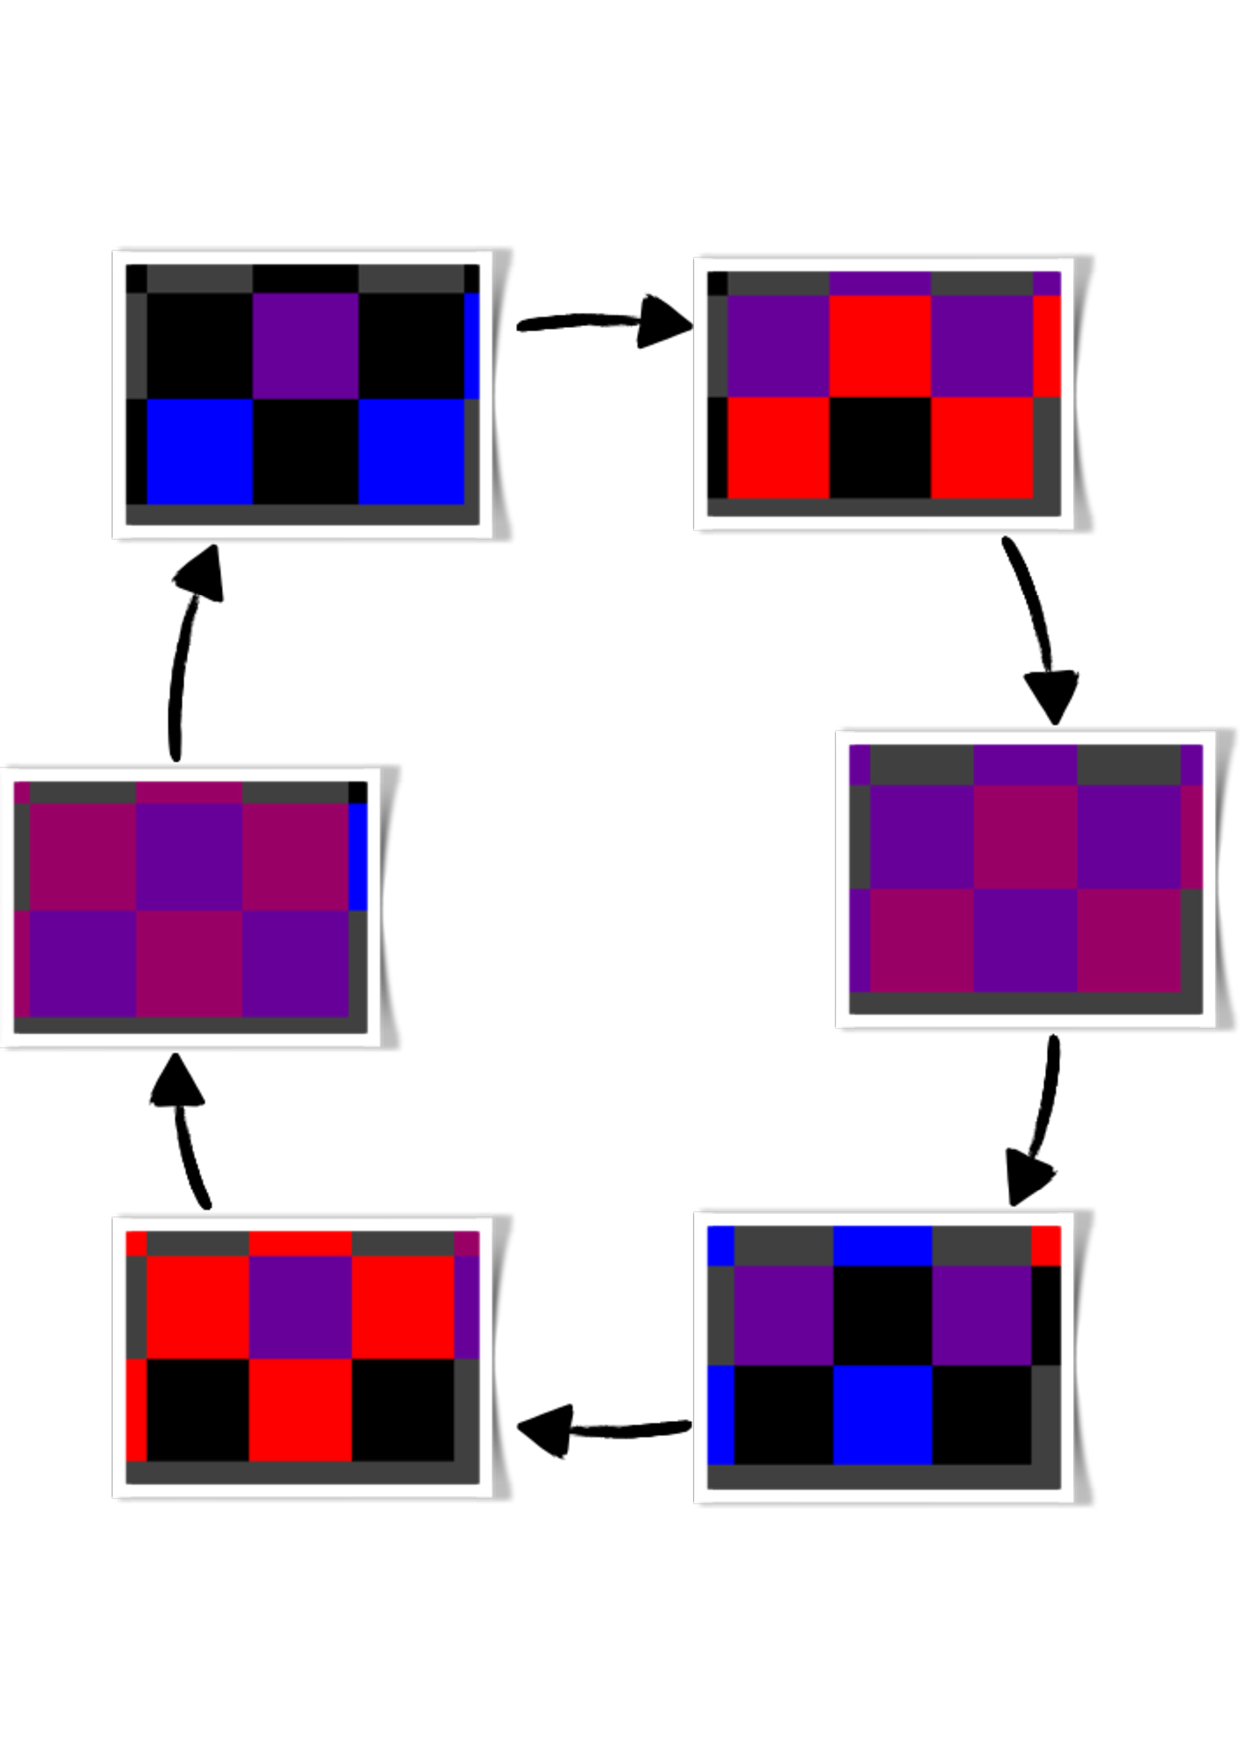
\includegraphics[width=0.45\columnwidth]{img/cyclesReal}\\
    (a) & (b)
\end{tabular}
\caption{\textbf{Six steps survival strategy}: (a) from a genotype extracted from a HetCA simulation in a stable environment and in a randomly initialized homogenous CA and (b) from a HetCA simulation with \emph{Short-cycle Fluctuations}. }
  \label{foursteps}
\end{figure}
 
%\begin{figure}[h]
%\centering
%\caption{\textbf{Six steps survival strategy} }
%  \label{fourstepsreal}
%\end{figure}








\section{Results}\label{sec:results}
\subsection{Genotype Size \& Genotype mutations}
Figure~\ref{fig:Size} shows genotype size under the various study conditions. The size is bounded (50 is the maximum size) and it limits the differences between those environments as most simulations converge towards this limit, however, one can clearly see here that \emph{Short-cycle Fluctuation} restrict the size of the genotypes while other forms of fluctuations do not appear to have any effect on genotype size. This size reduction could be a way to increase the impact of genotypic mutations on the phenotype. Indeed even if in LGP, when a mutation occurs, its effect is proportional to the size of the genotype, long genotype may enable redundancy information to stabilize the phenotype. Figure~\ref{fig:Size} depicts the amount of accumulated mutation of the most common individual. The amount of mutations separating the current most common individual from individuals created at initialization of the simulation. It is not surprising that more mutations are selected when there are environmental fluctuations\footnote{And those seem to depend more on the strength of these fluctuations than on their periodicity.} but we note that the proximity of strong fluctuation and Short Cycle fluctuations indicates that their genotype difference in size is not only explained by differences in the number of selected mutations.


\begin{figure}[h]
\centering
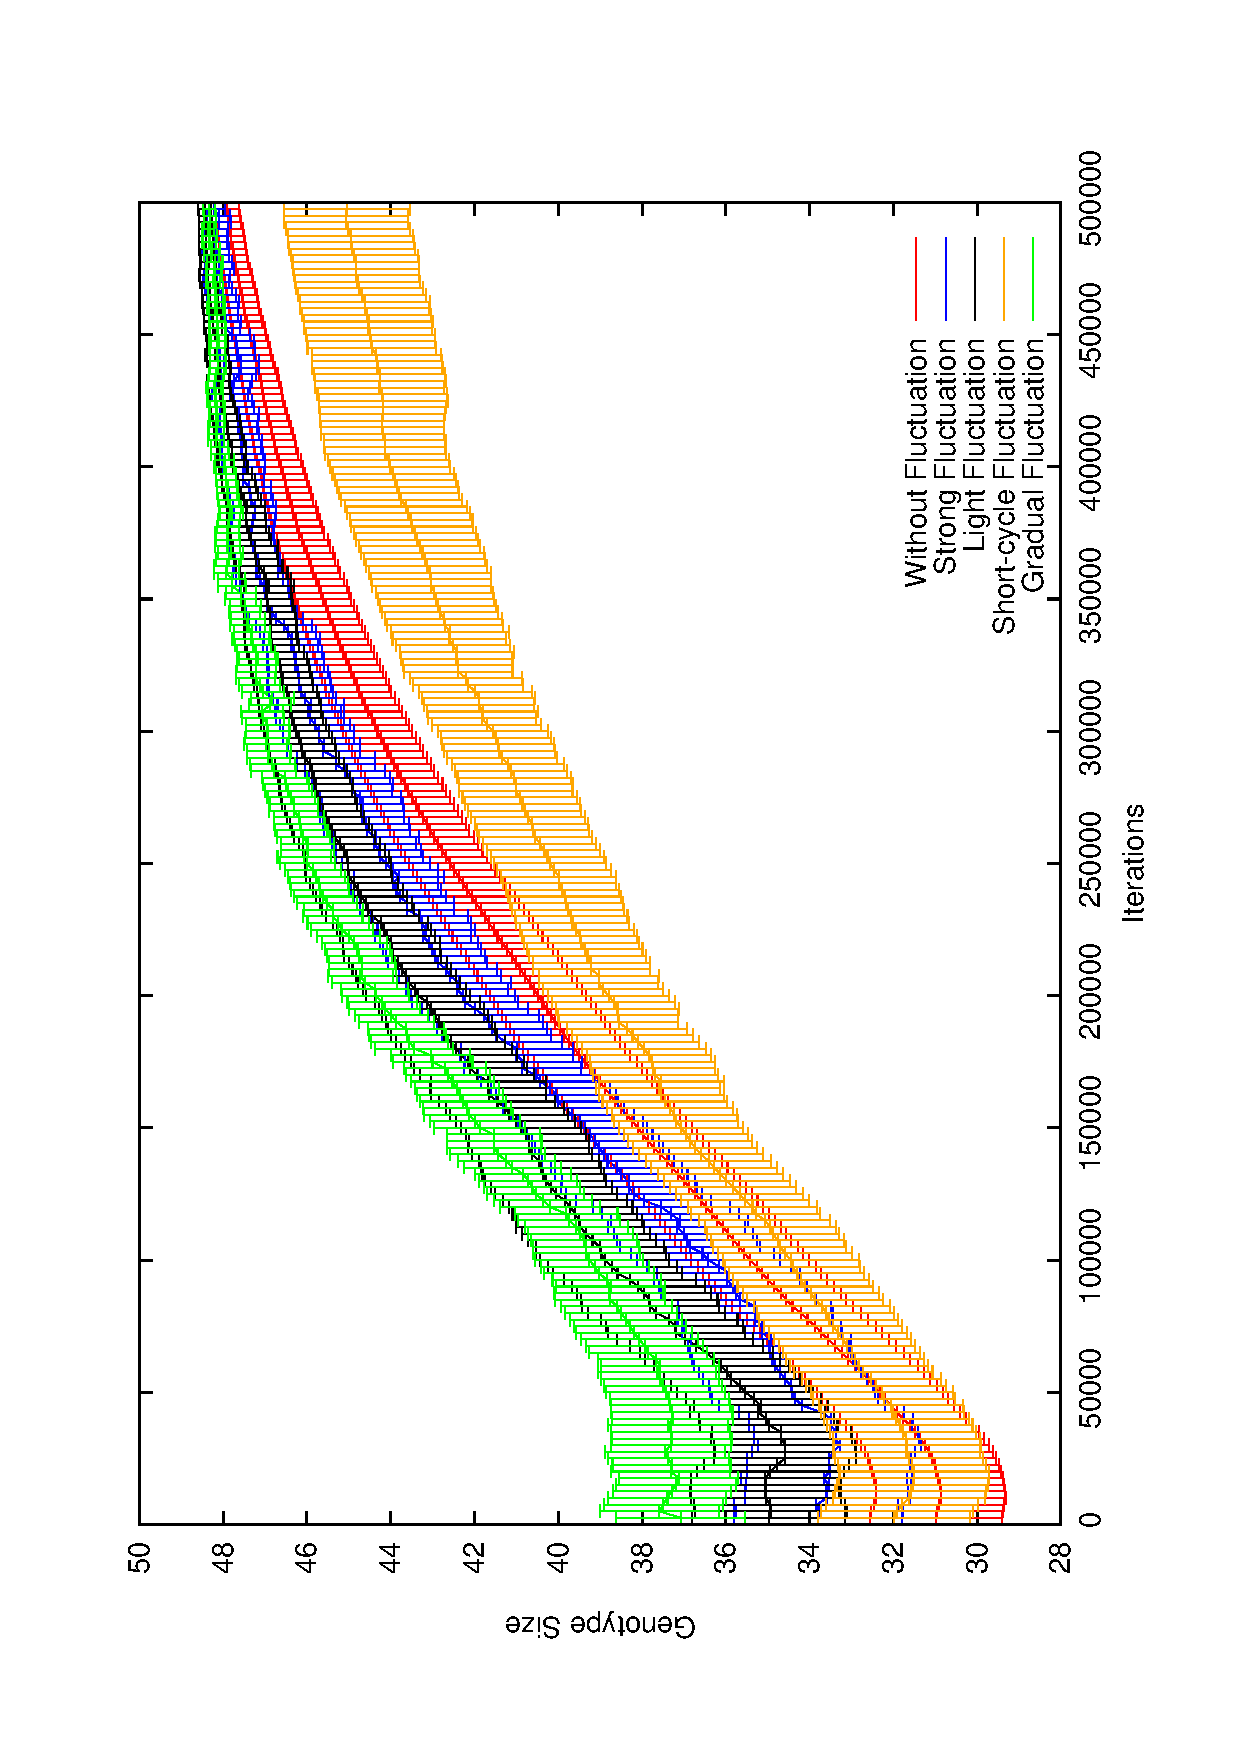
\includegraphics[width=0.7\columnwidth, angle =-90 ]{img/Size}
\caption{\textbf{Size of genotypes}. 
}
\label{fig:Size}
\end{figure}

\begin{figure}[h]
\centering
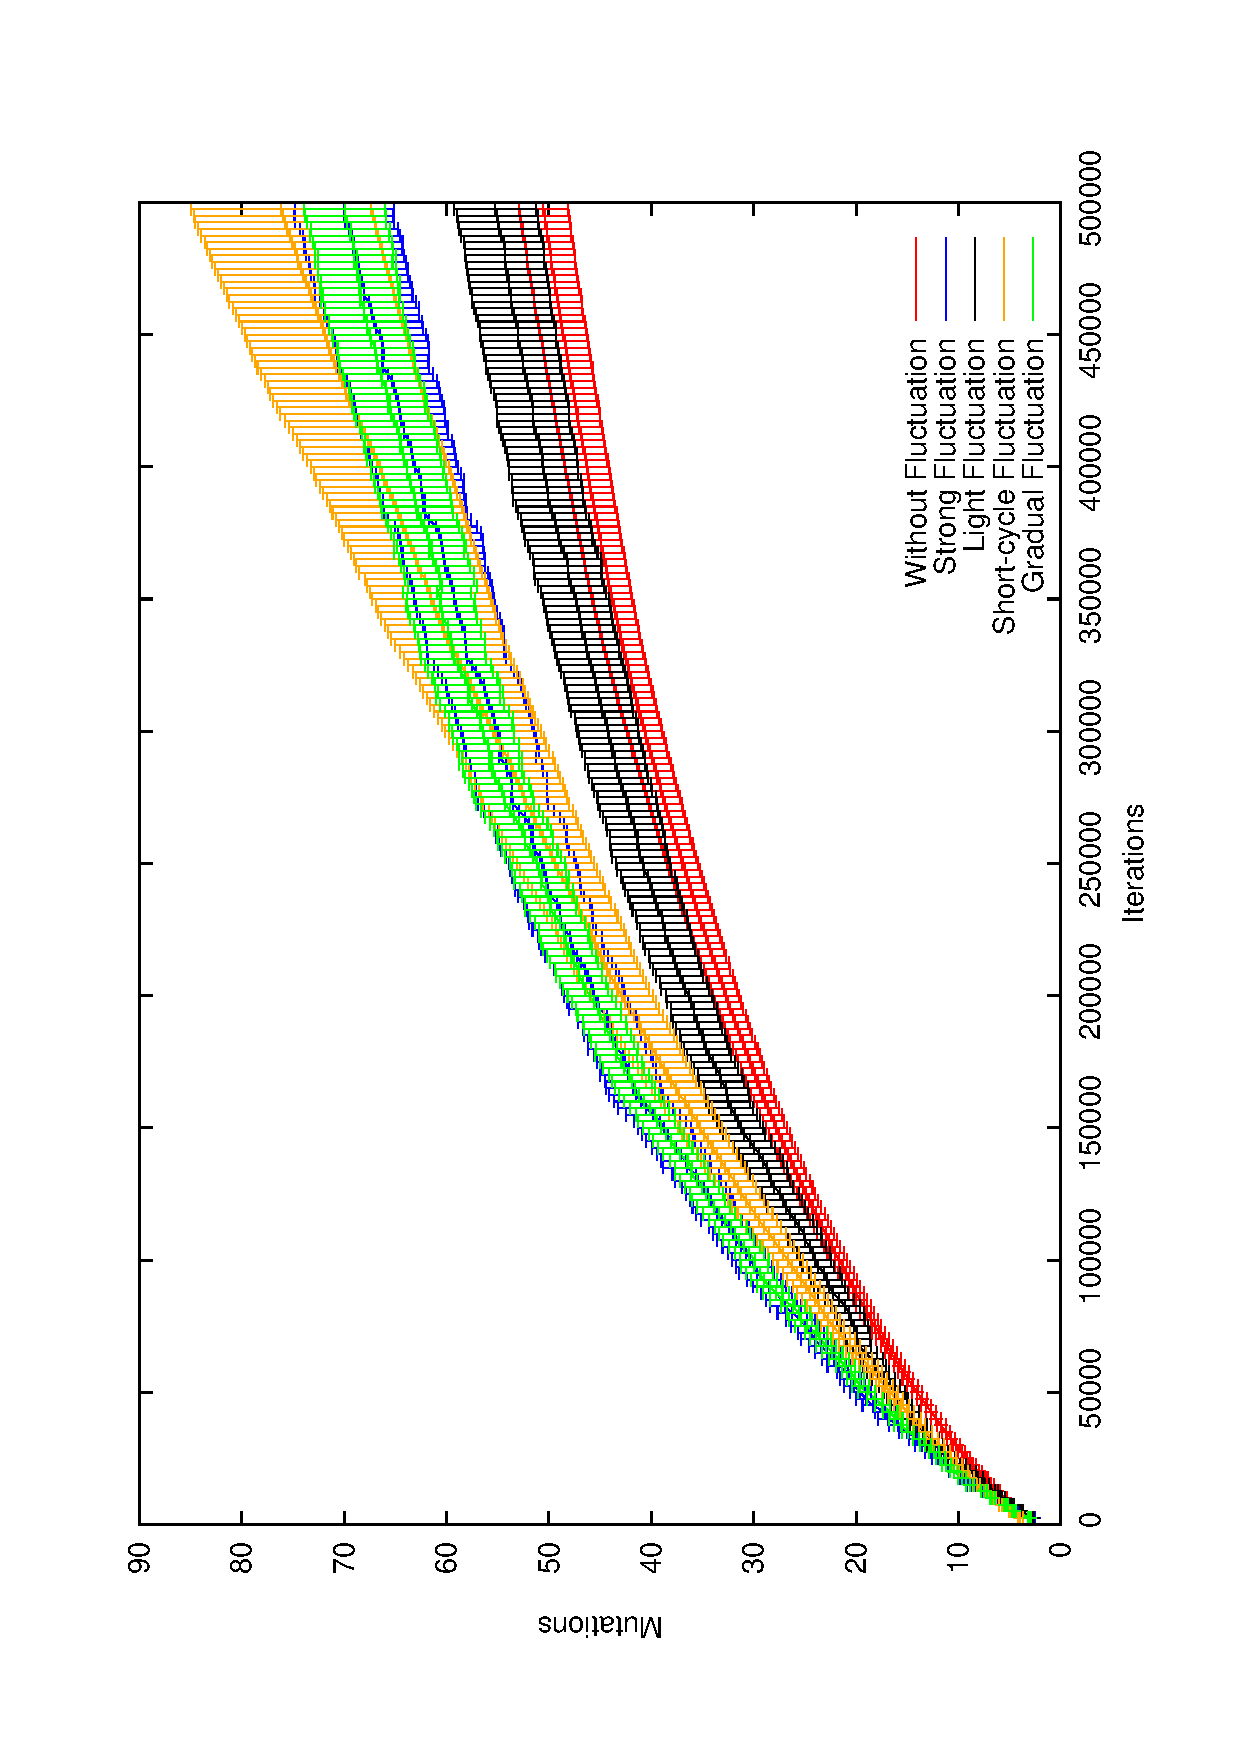
\includegraphics[width=0.7\columnwidth, angle =-90 ]{img/Mutations}
\caption{\textbf{Mutations of genotypes}.
}
\label{fig:Mutations}
\end{figure}

\subsection{Phenotypic Comparison}
Figure~\ref{fig:disimilar} depict phenotypic comparison of disimilar environment, one can see that the impact of environmental fluctuations decreases for \emph{Short-cycle  Fluctuation} while it remains very high for other forms of environmental fluctuations. We also noted that the phenotypic difference fall quickly for \emph{Short-cycle fluctuations} and even became almost similar to that of the simulation without fluctuation from iteration 20000. This suggests a selection of a single phenotype, robust in both environments. Figure~\ref{fig:disimilar} depict phenotypic comparison of similar environmen

\begin{figure}[h]
\centering
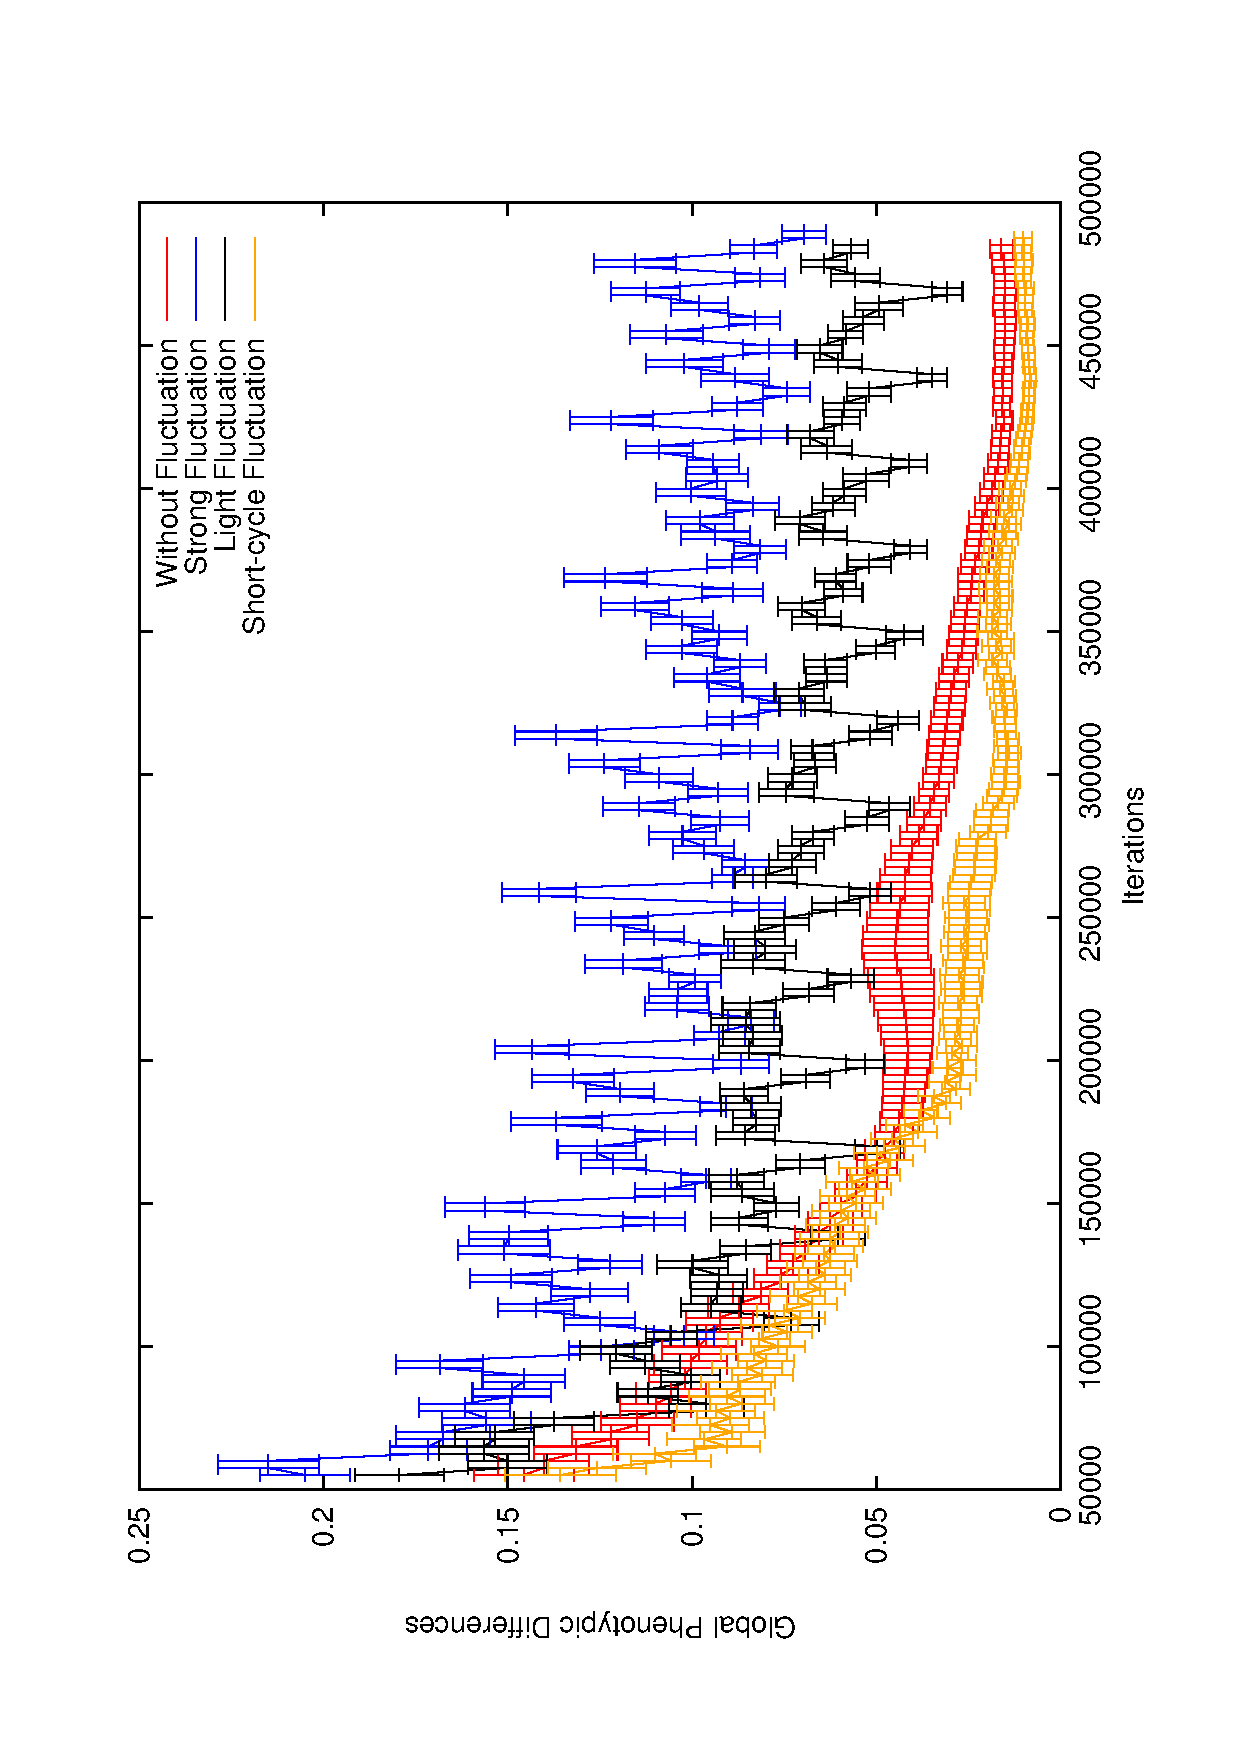
\includegraphics[width=0.7\columnwidth, angle =-90 ]{img/diffProp}
\caption{\textbf{phenotypic comparison of disimilar environment}.
}
\label{fig:disimilar}
\end{figure}

\begin{figure}[h]
\centering
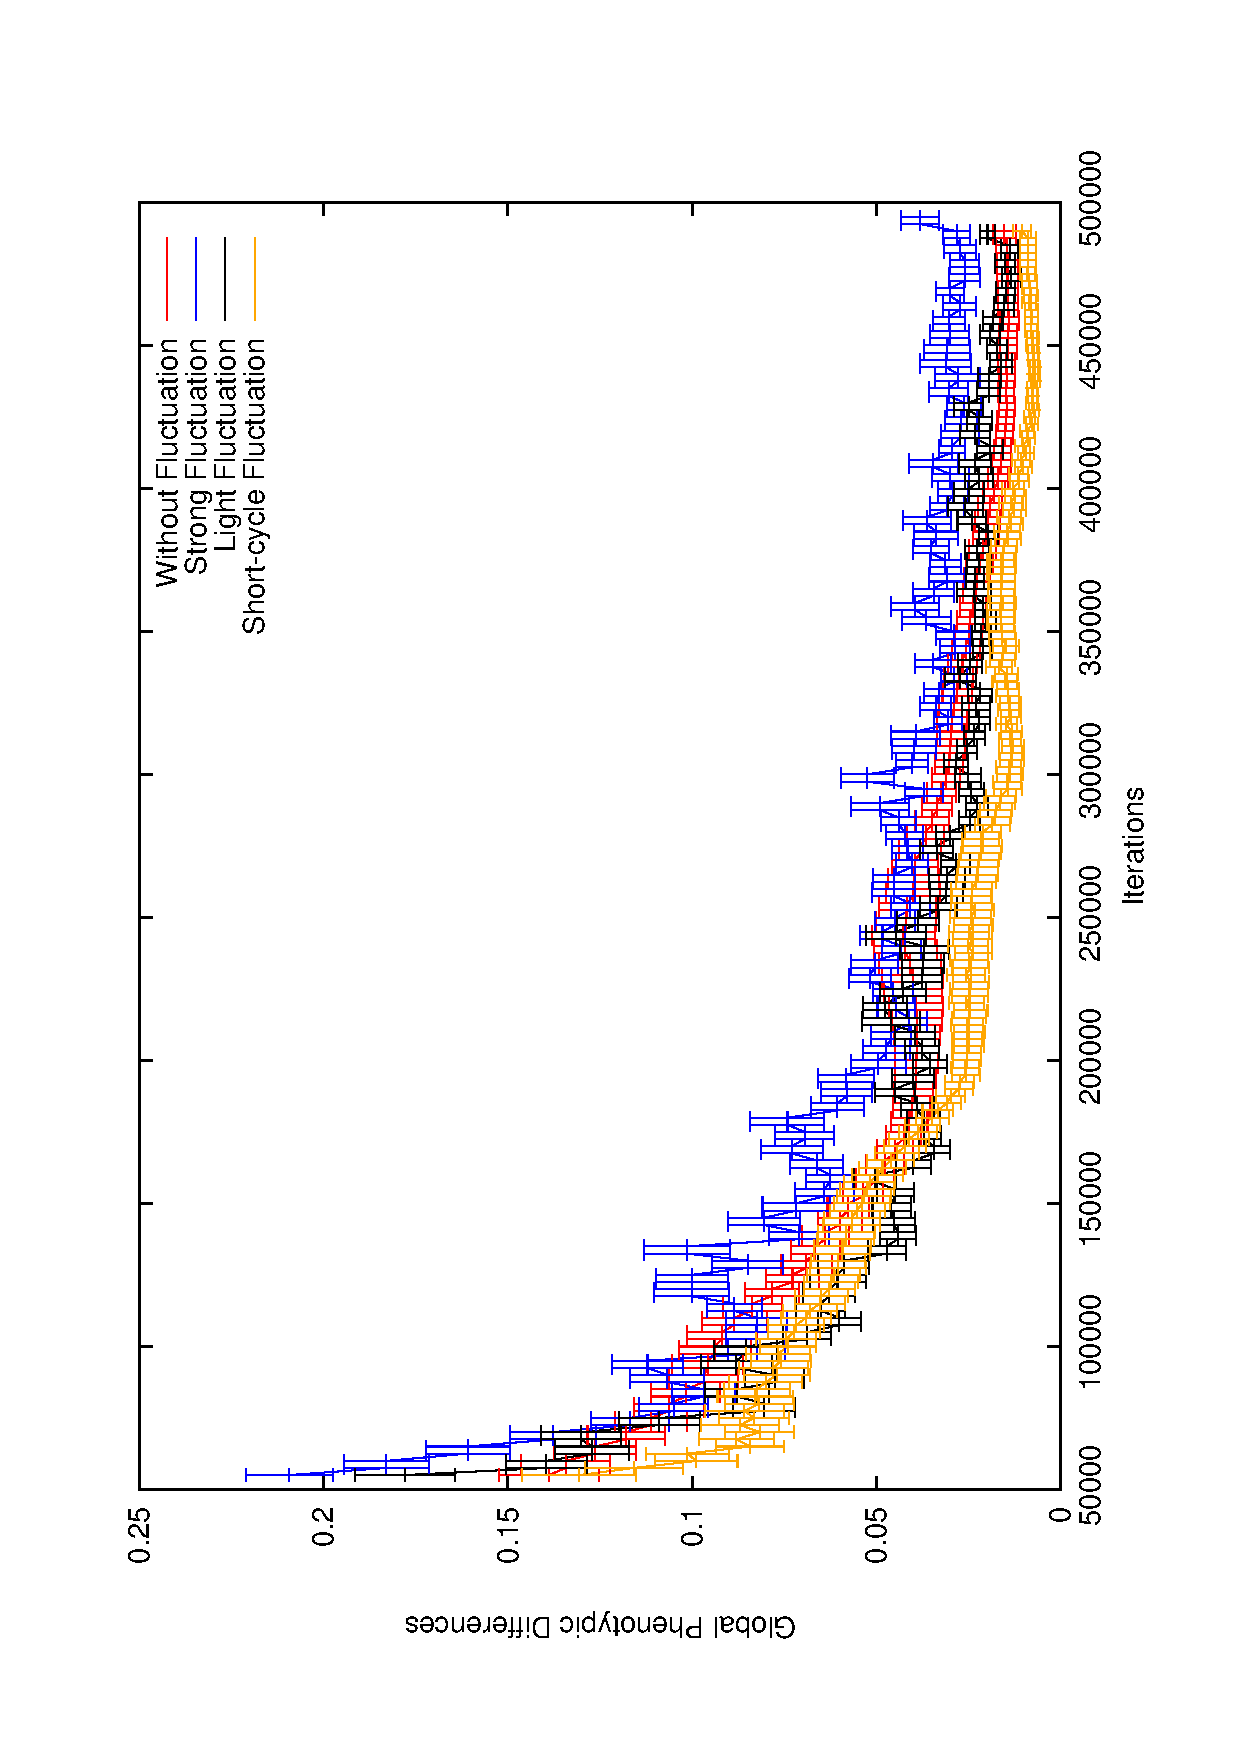
\includegraphics[width=0.7\columnwidth, angle =-90 ]{img/ProgressProp}
\caption{\textbf{phenotypic comparison of similar environment} : Here one can see that the impact of environmental fluctuations decreases for \emph{Short-cycle  Fluctuation} and  \emph{Light  Fluctuation}  while it remains very high for other forms of environmental fluctuations.
}
\label{fig:similar}
\end{figure}

\subsection{Success Rate end ending iteration of homogenous test}
Success rates of genotypes in different homogenous simulations are reported in Table \ref{tab:scstable} to \ref{tab:scstrong} using normal approximation interval with a confidence of 95\%. Looking at the different success rates we can first order the different tested environment by increasing difficulty : \emph{Stable Environment}; \emph{Short-cycle Fluctuations}; \emph{Light Fluctuations} ; \emph{Strong Fluctuations}. The fact that the \emph{stable environment} offers the lowest challenge is not surprising. Similarly the fact that \emph{Light Fluctuations} are less difficult than \emph{Strong fluctuations} is quite expected. We believe that the slightest difficulty in \emph{Short-cycle Fluctuations} than in \emph{Light Fluctuations} is due to the reduced number of different environment in \emph{Short-cycle Fluctuations} and, in particular, to the fact that, in this configuration, one of the living state is allowed for all environments $K(S_3)=1$. It is also noteworthy that individuals from \emph{Strong and Light Fluctuations} seem relatively robust in various environmental configurations while those from \emph{Short-cycle Fluctuations} doesn't seem robust outside environmental conditions in which they evolved. Moreover, among genotypes collected from iteration 102500, these same individuals are the only ones that do not reach a 100\% survival ratio in a stable environment.
 


\begin{table*}
\caption{Success Rate of genotypes in homogenous test with stable environment.\label{tab:scstable}}
\scriptsize
\begin{tabular}{ccccccc}
\toprule%
{\textbf{Collection}} & {\textbf{2500}} & \textbf{102500} & \textbf{202500} &\textbf{302500} &\textbf{402500} &\textbf{500000} \tabularnewline
\toprule%
\textbf{Stable Environment} & $88\%\pm9\%$ & $100\%\pm0\%$ & $100\%\pm0\%$ & $100\%\pm0\%$ & $100\%\pm0\%$ & $100\%\pm0\%$\tabularnewline

\textbf{Short-cycle Fluctuations} & $98\%\pm4\%$ & $88\%\pm9\%$ & $88\%\pm9\%$ & $88\%\pm9\%$ & $88\%\pm9\%$ & $88\%\pm9\%$\tabularnewline

\textbf{Light Fluctuations} & $94\%\pm6\%$ & $100\%\pm0\%$ & $100\%\pm0\%$ & $100\%\pm0\%$ & $100\%\pm0\%$ & $100\%\pm0\%$\tabularnewline

\textbf{Strong Fluctuations} & $96\%\pm5\%$ & $100\%\pm0\%$ & $100\%\pm0\%$ & $100\%\pm0\%$ & $100\%\pm0\%$ & $100\%\pm0\%$\tabularnewline

\bottomrule%
\end{tabular}%
\end{table*} 

\begin{table*}
\caption{Success Rate of genotypes in homogenous test with Short Cycle Fluctuations.\label{tab:scshort}}
\scriptsize
\begin{tabular}{ccccccc}
\toprule%
{\textbf{Collection}} & {\textbf{2500}} & \textbf{102500} & \textbf{202500} &\textbf{302500} &\textbf{402500} &\textbf{500000} \tabularnewline
\toprule%

\textbf{Stable Environment} & $37\%\pm13\%$ & $55\%\pm14\%$ & $45\%\pm14\%$ & $55\%\pm14\%$ & $57\%\pm14\%$ & $47\%\pm14\%$ \tabularnewline
\textbf{Short-cycle Fluctuations} & $33\%\pm13\%$ & $88\%\pm9\%$ & $88\%\pm9\%$ & $88\%\pm9\%$ & $88\%\pm9\%$ & $88\%\pm9\%$ \tabularnewline
\textbf{Light Fluctuations} &$29\%\pm13\%$ & $61\%\pm13\%$ & $69\%\pm13\%$ & $69\%\pm13\%$ & $84\%\pm10\%$ & $82\%\pm10\%$ \tabularnewline
\textbf{Strong Fluctuations} &$40\%\pm14\%$ & $80\%\pm11\%$ & $96\%\pm5\%$ & $96\%\pm5\%$ & $90\%\pm8\%$ & $86\%\pm9\%$\tabularnewline

\bottomrule%
\end{tabular}%
\end{table*} 

\begin{table*}
\caption{Success Rate of genotypes in homogenous test with Light Fluctuations.\label{tab:scslight}}
\scriptsize
\begin{tabular}{ccccccc}
\toprule%
{\textbf{Collection}} & {\textbf{2500}} & \textbf{102500} & \textbf{202500} &\textbf{302500} &\textbf{402500} &\textbf{500000} \tabularnewline
\toprule%

\textbf{Stable Environment} & $20\%\pm11\%$ & $59\%\pm14\%$ & $65\%\pm13\%$ & $73\%\pm12\%$ & $73\%\pm12\%$ & $67\%\pm13\%$\tabularnewline
\textbf{Short-cycle Fluctuations} & $18\%\pm10\%$ & $20\%\pm11\%$ & $14\%\pm9\%$ & $10\%\pm8\%$ & $8\%\pm7\%$ & $6\%\pm6\%$\tabularnewline
\textbf{Light Fluctuations} &$20\%\pm11\%$ & $90\%\pm8\%$ & $96\%\pm5\%$ & $98\%\pm4\%$ & $100\%\pm0\%$ & $98\%\pm4\%$\tabularnewline
\textbf{Strong Fluctuations} &$24\%\pm12\%$ & $90\%\pm8\%$ & $98\%\pm4\%$ & $96\%\pm5\%$ & $96\%\pm5\%$ & $100\%\pm0\%$\tabularnewline

\bottomrule%
\end{tabular}%
\end{table*} 

\begin{table*}
\caption{Success Rate of genotypes in homogenous test with Strong Fluctuations.\label{tab:scstrong}}
\scriptsize
\begin{tabular}{ccccccc}
\toprule%
{\textbf{Collection}} & {\textbf{2500}} & \textbf{102500} & \textbf{202500} &\textbf{302500} &\textbf{402500} &\textbf{500000} \tabularnewline
\toprule%

\textbf{Stable Environment} & $0\%\pm0\%$ & $16\%\pm10\%$ & $16\%\pm10\%$ & $14\%\pm9\%$ & $12\%\pm9\%$ & $12\%\pm9\%$\tabularnewline
\textbf{Short-cycle Fluctuations} & $0\%\pm0\%$ & $4\%\pm5\%$ & $2\%\pm4\%$ & $4\%\pm5\%$ & $0\%\pm0\%$ & $0\%\pm0\%$\tabularnewline
\textbf{Light Fluctuations} & $2\%\pm4\%$ & $16\%\pm10\%$ & $25\%\pm12\%$ & $29\%\pm13\%$ & $29\%\pm13\%$ & $45\%\pm14\%$\tabularnewline
\textbf{Strong Fluctuations} & $0\%\pm0\%$ & $31\%\pm13\%$ & $43\%\pm14\%$ & $55\%\pm14\%$ & $55\%\pm14\%$ & $55\%\pm14\%$\tabularnewline

\bottomrule%
\end{tabular}%
\end{table*} 

\subsection{Last iterations}

Figure \ref{fig:ending} depict the last iteration with living cells of homogenous runs that didn't reach 60000. Note that \emph{Short-cycle Fluctuation} genotypes failures are concentrated around iteration 15000 on \emph{Light Fluctuation} homogenous test and around iteration 25000 on \emph{Strong Fluctuation} homogenous test. This corresponds, for these two configurations, to the first environment for which $K(S_3)=0$, while $K(S_3)=1$ for every environment used in \emph{Short-cycle Fluctuation}. 

\begin{figure}[H]
\begin{subfigure}{.25\textwidth}
  \centering
  \includegraphics[width=.7\linewidth, angle =-90]{img/boxendingsFailedstable.eps}
  \caption{Stable environment.}
  \label{fig:sfig1}
\end{subfigure}%
\begin{subfigure}{.25\textwidth}
  \centering
  \includegraphics[width=.7\linewidth, angle =-90]{img/boxendingsFailedvariation.eps}
  \caption{Strong Fluctuation.}
  \label{fig:sfig2}
\end{subfigure}

\begin{subfigure}{.25\textwidth}
  \centering
  \includegraphics[width=.7\linewidth, angle =-90]{img/boxendingsFailedvariationLight.eps}
  \caption{Light Fluctuation.}
  \label{fig:sfig2}
\end{subfigure}%
\begin{subfigure}{.25\textwidth}
  \centering
  \includegraphics[width=.7\linewidth, angle =-90]{img/boxendingsFailedvariationSmall.eps}
  \caption{Small Fluctuation.}
  \label{fig:sfig1}
\end{subfigure}
\caption{Last iteration with living cells of homogenous runs that didn't reach 60000. iterations.}
\label{fig:ending}
\end{figure}

\begin{figure}[H]
\begin{subfigure}{.25\textwidth}
  \centering
  \includegraphics[width=.7\linewidth, angle =-90]{img/boxdensitystable.eps}
  \caption{Stable environment.}
  \label{fig:sfig1}
\end{subfigure}%
\begin{subfigure}{.25\textwidth}
  \centering
  \includegraphics[width=.7\linewidth, angle =-90]{img/boxdensityvariation.eps}
  \caption{Strong Fluctuation.}
  \label{fig:sfig2}
\end{subfigure}

\begin{subfigure}{.25\textwidth}
  \centering
  \includegraphics[width=.7\linewidth, angle =-90]{img/boxdensityvariationLight.eps}
  \caption{Light Fluctuation.}
  \label{fig:sfig2}
\end{subfigure}%
\begin{subfigure}{.25\textwidth}
  \centering
  \includegraphics[width=.7\linewidth, angle =-90]{img/boxdensityvariationSmall.eps}
  \caption{Small Fluctuation.}
  \label{fig:sfig1}
\end{subfigure}
\caption{Density of Genotype : Each genotype density is processed in four possible different environments.}
\label{fig:size}
\end{figure}

\section{Analysis}
\subsection{Environmental Transitions} 
Figure \ref{fig:trans} depicts the average transition between environments in different homogenous runs. To compute this typical transition we averaged phenotype disturbance calculated at iterations $[t-40; t + 40] \forall t \in T_r	
\ge 5000$ where $T_r$ is the set of every iteration of the run $r$ such that a transitions between environments occurs, i.e. $E(t) \ne E(t+1)$. Figure  \ref{fig:transonly} shows the different average transitions of ScF genotypes tested a homogeneous test with the same fluctuations. We can see that phenotypes of the genotypes collected later in the evolutionary process are less sensitive to environmental fluctuations. Conversely, as reported of Figure \ref{fig:transli}, the phenotypes of genotypes from SF keep the same high sensitivity regardless of the iteration in which they were collected. Finally the figures \ref{fig:transst} and \ref{fig:transstest} compare the average transitions in homogeneous test with ScF and SF of genotypes collected at iteration 500000 in the four different configurations. Again, it can be seen there that the phenotype of ScF is much more stable than others in its original environment. On the contrary, tested in SF this genotype is very sensitive to transitions. High sensitivity to fluctuations includes both individuals which developed plasticity and those which fail to resist the environement fluctuations.


\begin{figure}[H]
\begin{subfigure}{.25\textwidth}
  \centering
  \includegraphics[width=.7\linewidth, angle =-90]{img/Sucavg499999variationb.eps}
  \caption{SF on genotypes from i:50000.}
  \label{fig:transst}
\end{subfigure}%
\begin{subfigure}{.25\textwidth}
  \centering
  \includegraphics[width=.7\linewidth, angle =-90]{img/SucavgvarValidvariationb.eps}
  \caption{SF on genotypes from SF.}
  \label{fig:transli}
\end{subfigure}

\begin{subfigure}{.25\textwidth}
  \centering
  \includegraphics[width=.7\linewidth, angle =-90]{img/Sucavg499999variationSmallb.eps}
  \caption{ScF on genotypes from i:50000.}
  \label{fig:transstest}
\end{subfigure}%
\begin{subfigure}{.25\textwidth}
  \centering
  \includegraphics[width=.7\linewidth, angle =-90]{img/SucavgvarSmallValidvariationSmallb.eps}
  \caption{ScF on genotypes from ScF.}
  \label{fig:transonly}
\end{subfigure}
\caption{\textbf{phenotype disturbance} : Average transition between environment in different types of homogenous test.}
\label{fig:trans}
\end{figure}


\subsection{Phenotypic Diversity} 



\begin{figure}
\begin{subfigure}{.25\textwidth}
  \centering
  
\includegraphics[width=.9\linewidth]{img/stable495000}
  \caption{SE}
\end{subfigure}%
\begin{subfigure}{.25\textwidth}
  \centering
  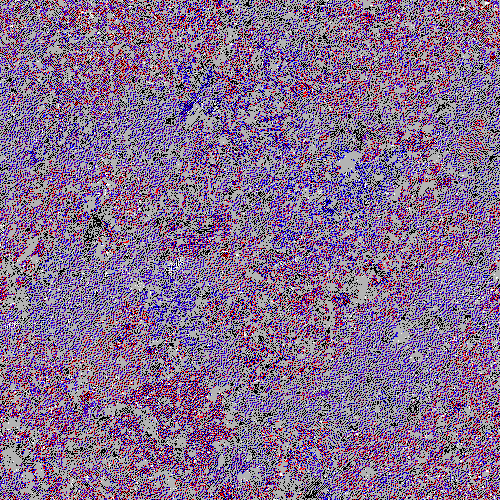
\includegraphics[width=.9\linewidth]{img/var495000}
  \caption{SF}
\end{subfigure}

\begin{subfigure}{.25\textwidth}
  \centering
  
\includegraphics[width=.9\linewidth]{img/light495000}
  \caption{LF}
\end{subfigure}%
\begin{subfigure}{.25\textwidth}
  \centering
  
\includegraphics[width=.9\linewidth]{img/small495000}
  \caption{ScF}
\end{subfigure}
\caption{\textbf{Example of CA} gird state repartition (phenotype) at iteration 495000 for the four different configuration. Each cell state is represented by a different color. Black and grey represent respectively cells in \emph{decay} and \emph{quiescent} state.}
\label{fig:phenoexpl}
\end{figure}

The phenotypic diversity measured in Figure \ref{fig:phenodiv} can also be observed relatively easily by simple observation of the cellular automaton as it can be seen with a few examples in Figures \ref{fig:phenoexpl}. 


One distinguishes LF and SF from ScF. These two groups diverge substantially in their characteristic and differ in addition from SE. Individuals from ScF seem to produce stable and robust phenotypes in any environment encountered in ScF. Their adaptations seem essentially be by genotypic mutations and their plasticity seems low. They are also very dependent on their original ecosystem, sometime very distinctive as depicted in Figure \ref{fig:smalldistinctive}, and consequently very little robust in other types of fluctuations, the effect of genotypic mutations is probably enhanced by the reduced size of genotypes. By contrast individuals evolved with LF or SF appear to have a considerable plasticity, their phenotypic diversity is high and it seems likely that phenotypic selection occurs however their genotypic diversity is lower.

\begin{figure}
\begin{subfigure}{.12\textwidth}
  \centering
  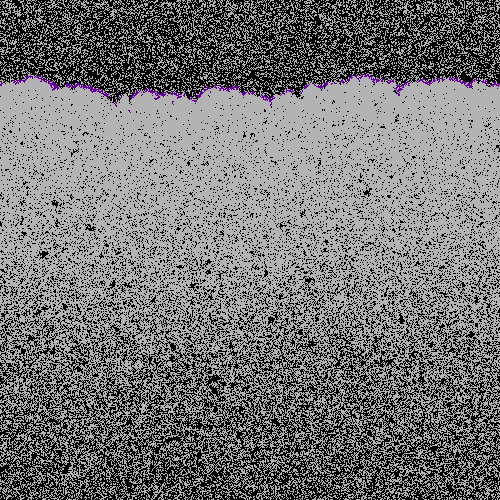
\includegraphics[width=1\linewidth]{img/sm100000}
  \caption{$t=100000$}
\end{subfigure}%
\begin{subfigure}{.12\textwidth}
  \centering
  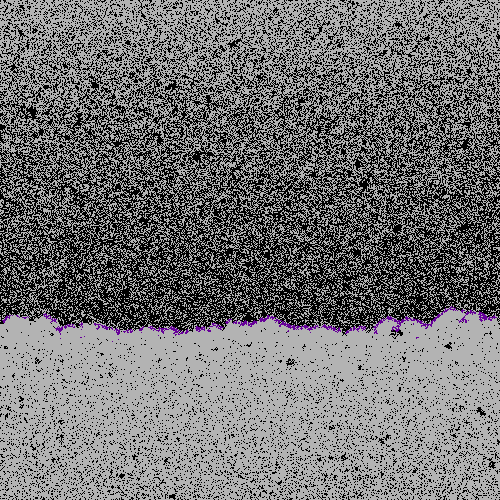
\includegraphics[width=1\linewidth]{img/sm200000}
  \caption{$t=200000$}
\end{subfigure}%
\begin{subfigure}{.12\textwidth}
  \centering
  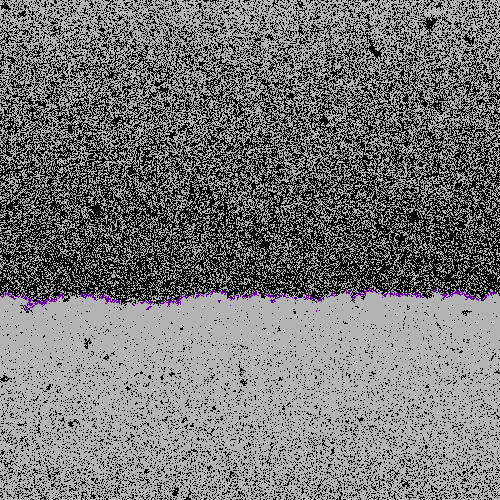
\includegraphics[width=1\linewidth]{img/sm400000}
  \caption{$t=400000$}
\end{subfigure}%
\begin{subfigure}{.12\textwidth}
  \centering
  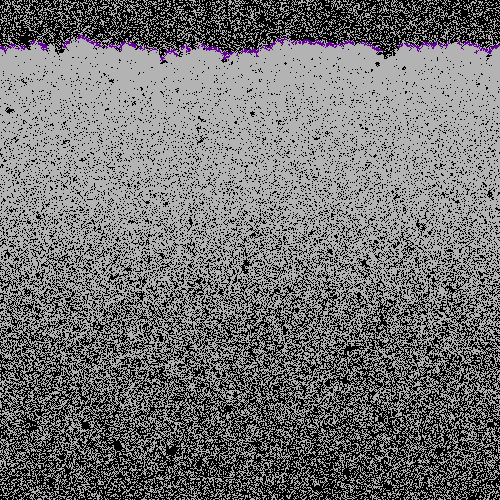
\includegraphics[width=1\linewidth]{img/sm500000}
  \caption{$t=500000$}
\end{subfigure}
\caption{\textbf{Original ScF simulation} having a distinctive waving phenotype, very stable over time $t$, and producing genotypes failing in early iteration of homogeneous test.}
\label{fig:smalldistinctive}
\end{figure}


\section{Conclusions}\label{sec:conc}
Plasticity, phenotypic diversity and phenotypic selection are all evolutionary properties that are found in this series of simulations, and evoke the multilevel selection model described by~\citet{jablonka2014evolution}. Among the three tested environmental fluctuations, the LF and SF simulations are showing the most similarities with this model. In ScF, the most successful evolutionary strategy seems to involve small genotypes, which could be favored for their ability to maximize the phenotypic impact of mutations. Furthermore, the inability of most ScF individuals to survive outside of the ecosystem resulting from their evolutionary history is reminiscent of the impossibility of saving species by the unique preservation of their DNA mentioned in \cite{jablonka2014evolution}: \say{You would have to reconstruct the community, and often these communities are very old, with historical memories that are stored in their epigenetic and behavioral systems. These are part of their ``identity,'' part of their stability. You cannot freeze these memories: they have to be maintained and transmitted through use, so you cannot reconstruct the communities from their component parts.} (\emph{ibid.},~p.~363). However, these experiments cannot determine whether the main indicator of differences between LF and SF one side and ScF on the other side is the duration of the environmental cycles or the number of different types of environments, and further investigation is needed.

\section{Acknowledgement}
Funding for this work was provided by the Science Foundation Ireland and ERC Advanced Grant EPNet (340828).
Some of the simulations have been done in the supercomputer MareNostrum at Barcelona Supercomputing Center.
\bibliography{David,Simon}
\bibliographystyle{apalike}
\end{document}
